\documentclass[oneside,a4paper,10pts,article]{memoir}

\usepackage{palatino}
\usepackage{graphicx}
\usepackage{todonotes}

\title{Tradeable Certificates of Title on a blockchain \\
 {\normalfont\normalsize\scshape A case study on a trust-free vehicle registry}
}
\author{Martin Dybdal \texttt{dybber@dybber.dk}}
\date{\today}

\begin{document}

\maketitle

\chapter{Preface}
This report was written as part of the ``Blockchain Summer School
2016'', which was held at the IT University of Copenhagen, August
2016. At the summer school we were allocated into groups and assigned
a case, that we needed to solve using blockchain
technology. Group-members: Felix Albert, Jacob Cholewa, Arun Prasad,
Benedikt Notheisen, Martin Dybdal.

\chapter{Introduction}
Blockchain technology provides a decentralised database infrastructure
which is tamper-proof and trust-free. In essence, a blockchain is a
distributed, append-only digital ledger, which can be trusted, as
transactions are validated by all the nodes in the network and is made
tamper-proof by the use of hashing algorithms. We call blockchain
trust-free, as you do not need to trust any individual parties (such
as when you trust your bank), the trust is generated by the
contruction of the network. A more detailed introduction to
blockchains is found in Section \ref{sec:blockchain}.

Blockchain technology is said to revolutionise businesses in domains
such as finance, logistics and administration, as documents,
contracts, certificates and so on, can be fully digitalised. In this
project we have worked on a case arising in public sector
administration, on the documentation and trust issues involved in
vehicle registration, vehicle taxation and vehicle trading. The Danish
Tax Agency (SKAT) is responsible for administering the registry of
danish motor vehicles, and provided us with thorough case description,
as well as support on aspects on the danish vehicle
registration-process during the summer school.

We have developed a small-prototype system, which can represent a
Vehicle Title (dan. registreringsattest) as a tradeable contract on
the blockchain system called Ethereum. The aspect of ownership change
is a core problem in the digitalization of Vehicle Title. In Section
\ref{sec:case} we will detail the major steps in Vehicle registration
and taxation in Denmark. In Section \ref{sec:trading} we describe the
core problems of trading contracts, and how it can be solved using a
blockchain. In Section \ref{sec:currency} we look at the problem of
representing non-crypto currencies, such as Danish Kroner or Euro's in
a blockchain. In Section \ref{sec:implementation} we describe our
Ethereum prototype and in Section \ref{sec:futurework} and
\ref{sec:conclusion} we describe future prospects and conclude.

\chapter{Case description}
\label{sec:case}
Registration of vehicles, collecting vehicle taxes, and interacting
with other stakeholders, such as police, insurance companies and
transport authorities, requires a lot of administration, and a lot of
things can go wrong in process.

\section{The lifecycle of a vehicle}
During the lifecycle of vehicle, it goes through various owners and
activities, and involves several different parties, such as car
importers, police, insurance companies, MOT Testing companies and
transport authorities. When a car is imported into the country, it is
registered as owned by the importer, which sells it to a specific
dealer. The dealer then sells it to a private owner or a corporation,
and the car can be re-sold multiple times. See Figure \ref{fig:lifecycle}.

A crucial aspect is thus the change of ownership, which is registered
in the Danish Motor Registry. Especially the current process enforced
when trading used cars is problematic, as there is an imbalance of
knowledge and trust between the seller and the buyer. The buyer might
not know the full history of owners, accidents or repairs, and as the
Vehicle Title is currently on paper, it might be forged or the car
might be stolen. On the other hand, the seller has to put trust in the
buyer, that he will in fact re-register the car in his own
name. Currently, if the buyer does not immediately re-register the
car, the sellers insurance might still be covering damages and the
buyer could use the criminal activities, without being recorded as the
owner of the car.

This means that activities such as MOT Test, repairs and accident
reports are crucial for the buyer, and for the seller the
re-registration should be a part of the shift of ownership.

\begin{figure}
  \centering
  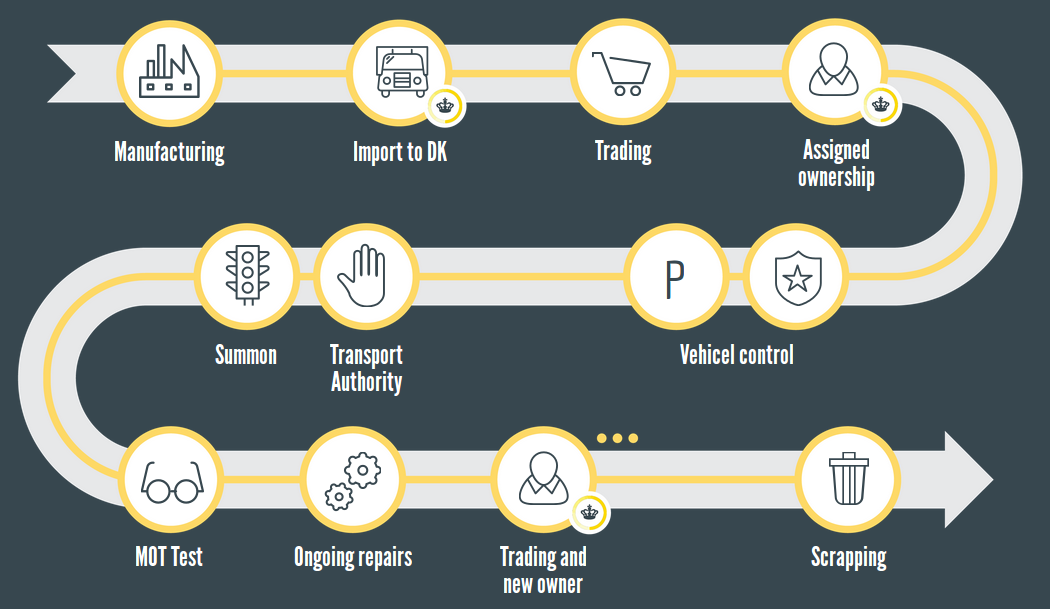
\includegraphics[width=\textwidth]{lifecycle.png}
  \caption{Vehicle Lifecycle}
  \label{fig:lifecycle}
\end{figure}

\section{Vehicle taxation in Denmark}
Taxation-wise there are several places where the Tax Agency needs to
be involved. When a car is imported, it has to be registered and a
registration tax has to be paid, it does not matter whether the car is
new or used. When a car shifts hands, the Tax Agency needs to know, as
they collect a yearly ownership tax for car owners. Also, several fees
can be levied as part of the process, for example a re-registration
fee. It is also the Tax Agency's job to make sure that all registered
cars are insured by their owner.

\section{Core challenges}
As outlined in the description above, the core challenges are:

\begin{itemize}
\item Giving buyer knowledge of vehicle history, which he can trust
\item Giving seller trust, that the buyer will not commit fraud
\item Ensuring that ownership taxes are collected from the rightful
  owner of the vehicle
\end{itemize}

\chapter{Blockchain}
\label{sec:blockchain}
An introduction to blockchain, both technical and the potential impact
of the technology

\chapter{Trading contracts}
\label{sec:trading}
As described in Section \ref{sec:case}, the main underlying challenge
is the transfer of ownership between a seller and a buyer. This
ownership is represented by a contract, a so called Certificate of
Title or in the case of a vehicles, a Vehicle Title. Trading a
vehicle, thus really means trading the Vehicle Title, stating who is
the rightful owner. In this section we will describe the current
process of such a trade, and we will describe how a blockchain
solution, can mitigate most of the current problems.

\todo{describe how a contract is traded today}

\todo{describe how a contract might be traded using blockchain}


This can be generalized, and instead talking about the specific case
of trading a vehicle, we can use the same framework for trading any
contract.


\chapter{Representing non-crypto currencies}
\label{sec:currency}
Describe that we assume a central bank will be willing to issue a
token contract, such that owners of Tokens on the blockchain can
convert such tokens back to actual danish kroner.

\chapter{Implementation}
\label{sec:implementation}

\section{Ethereum}

\section{Experience using Ethereum}
Describe how horrible the development environment is, how bad the
documentation is, and how terrible the error messages are.

Mention that Ethereum currently is good for prototyping, nothing else. 

Eventually a better language than Solidity may be introduced, but
currently not a good platform for any serious projects.

Mention Certified contract languages, such as the work by Tom Hvitved
or Patrick Bahr.

\chapter{Future work}
\label{sec:futurework}

\begin{itemize}
\item Proof of work, proof of stake, proof of space?
\item Can a system built now, be migrated to another system?
\item How much should be stored off the blockchain?
\item Prospect of using a more formaly defined contract specification language
\end{itemize}

\chapter{Conclusion}
\label{sec:conclusion}


\end{document}